\question{10.13}{
    Het aantal brandmeldingen dat in een stad per week is geregistreerd gedurende een periode van $100$ weken blijkt uit de tabel.
    Toets of het aantal branden per week is te beschouwen als een kansvariabele die een Poissonverdeling volgt met $\mu = 1$ (kies $\alpha = 0,05$).
    \begin{center}
        \begin{tabular}{cc}
            \toprule
                {\bfseries Aantal branden per week} & {\bfseries Frequentie} \\
            \cmidrule{1-1} \cmidrule{2-2}
                $0$ & $48$ \\
                $1$ & $24$ \\
                $2$ & $16$ \\
                $3$ & $8$ \\
                $4$ of meer & $4$ \\
            \cmidrule{1-1} \cmidrule{2-2}
                Totaal & $100$ weken \\
            \bottomrule
        \end{tabular}
    \end{center}
}
\answer{
    Omdat we willen kijken of de gegeven data overeenkomen met een specifieke discrete kansverdeling, in dit geval de Poissonverdeling met $\mu=1$, kunnen we een chikwadraattoets voor aanpassing (goodness-of-fit test) uitvoeren.
    Laat $X$ een kansvariabele zijn die het aantal branden telt in een willekeurige week.
    Verder is gegeven dat over een periode van $100$ weken het aantal branden is geteld.
    Bij een chikwadraattoets voor aanpassing beginnen we met het defini\"eren van de nulhypothese $H_0$ en de alternatieve hypothese $H_1$.

    \begin{align*}
        H_0: &\qquad \text{$X$ is Poisson verdeeld met gemiddelde $\mu=1$.} \\
        H_1: &\qquad \text{$X$ is NIET Poisson verdeeld met gemiddelde $\mu=1$.}
    \end{align*}

    Het significantieniveau $\alpha=0,05$ is gegeven in de opdracht, net als de geobserveerde data.
    Om de toetsingsgrootheid $X^2$ te kunnen bepalen, moeten we eerst de \emph{expected}-tabel berekenen.
    Omdat onder de nulhypothese $H_0$ geldt dat $X \sim \text{Poisson}(\mu=1)$, kunnen we deze verwachte aantallen uitrekenen. 
    Omdat we $100$ afzonderlijke weken bekijken, moet dit ook worden meegenomen in de verwachte frequenties.   
    \begin{center}
        \renewcommand{\arraystretch}{1.25}
        \begin{tabular}{ccc}
            \toprule
                {\bfseries Aantal branden} & {\bfseries Frequentie} & {\bfseries Frequentie} \\
                {\bfseries per week} & {\bfseries (observed)} & {\bfseries (expected)} \\
            \cmidrule{1-1} \cmidrule{2-2} \cmidrule{3-3}
                $0$         & $48$ & $100 \cdot \poissonpdf(\mu=1; k=0) = 36,7879$ \\
                $1$         & $24$ & $100 \cdot \poissonpdf(\mu=1; k=1) = 36,7879$ \\
                $2$         & $16$ & $100 \cdot \poissonpdf(\mu=1; k=2) = 18,3940$ \\
                $3$         &  $8$ & $100 \cdot \poissonpdf(\mu=1; k=3) = 6,1313$ \\
                $4$ of meer &  $4$ & $100 - 36,7879 - 36,7879 - \ldots = 1,8988$ \\
            \cmidrule{1-1} \cmidrule{2-2} \cmidrule{3-3}
                Totaal & $100$ dagen & $100$ dagen \\
            \bottomrule
        \end{tabular}
    \end{center}
    Merk op dat we de chikwadraatverdeling enkel konden gebruiken zodra de verwachte frequenties allemaal minstens $5$ zijn.
    Om dit te bereiken, moeten we categorie\"en samenvoegen, namelijk $3$ en $4$ of meer:
    \begin{center}
        \renewcommand{\arraystretch}{1.25}
        \begin{tabular}{ccc}
            \toprule
                {\bfseries Aantal branden} & {\bfseries Frequentie} & {\bfseries Frequentie} \\
                {\bfseries per week} & {\bfseries (observed)} & {\bfseries (expected)} \\
            \cmidrule{1-1} \cmidrule{2-2} \cmidrule{3-3}
                $0$         & $48$ & $36,7879$ \\
                $1$         & $24$ & $36,7879$ \\
                $2$         & $16$ & $18,3940$ \\
                $3$ of meer & $12$ & $8,0301$ \\
            \cmidrule{1-1} \cmidrule{2-2} \cmidrule{3-3}
                Totaal & $100$ dagen & $100$ dagen \\
            \bottomrule
        \end{tabular}
    \end{center}

    De toetsingsgrootheid $X^2$ bepalen we aan de hand van de volgende formule:

    \begin{align*}
        X^2  &= \sum_{i} \frac{(O_{i} - E_{i})^2}{E_{i}},
    \end{align*}

    waarbij $i = 1,2,3,4$ de index van de rij is.
    Dit geeft in dit specifieke geval een geobserveerde toetsingsgrootheid 
    
    \begin{align*}
        \chi^2  &= \sum_{i} \frac{(O_{i} - E_{i})^2}{E_{i}} \\
                &=\frac{(O_{1} - E_{1})^2}{E_{1}} + \frac{(O_{2} - E_{2})^2}{E_{2}} + \frac{(O_{3} - E_{3})^2}{E_{3}} + \frac{(O_{4} - E_{4})^2}{E_{4}} \\
                &= \frac{(48 - 36,7879)^2}{36,7879} + \frac{(24-36,7879)^2}{36,7879} + \frac{(16-18,3940)^2}{18,3940} + \frac{(12-8,0301)^2}{8,0301} \\
                &\approx 10,1366
    \end{align*}

    Onder de nulhypothese volgt de toetsingsgrootheid $X$ een chikwadraatverdeling met
    \[
        \text{df} = (\#\text{categorie\"en}-1) = 4 - 1 = 3
    \]
    vrijheidsgraden.

    Extreem grote waarde van de toetsingsgrootheid duiden op grote verschillen tussen observed en expected frequenties, dus het kritieke gebied is van de vorm $[g, \infty)$.
    Deze grenswaarde $g$ is de oplossing van de vergelijking
    \begin{align*}
        \chi^2\text{cdf}(\text{lower}=g; \text{upper}=10^{10}; \text{df}=3) = \alpha = 0,05
    \end{align*}
    De solver optie geeft $g \approx 7,8147$.
    Aangezien de toetsingsgrootheid $\chi^2$ groter dan deze grenswaarde is ($10,1366 > 7,8147$), geldt dat de toetsingsgrootheid in het kritieke gebied ligt en dus $H_0$ wordt verworpen.
    Er is voldoende bewijs om aan te nemen dat het aantal branden per week niet een Poissonverdeling met gemiddelde $\mu=1$ volgt.
    
    \begin{center}
        \resizebox{0.9\textwidth}{!}{
            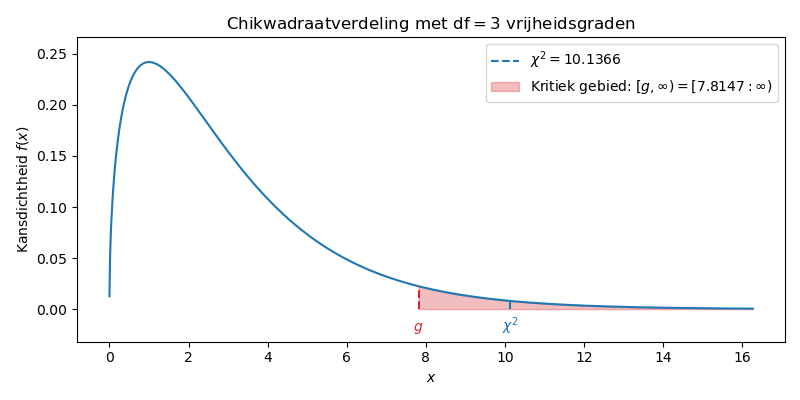
\includegraphics{opg_10.13_kritiek.png}
        }
    \end{center}

    {\bfseries Alternatief:} de $p$-waarde (rechteroverschrijdingskans) die hoort bij deze geobserveerde toetsingsgrootheid $\chi^2$ is gelijk aan
    \begin{align*}
        p   &= P(X^2 \ge \chi^2) \\
            &= \chi^2\text{cdf}(\text{lower}=\chi^2\approx 10,1366; \text{upper}=10^{10}; \text{df}=3) \\
            &\approx 0.0174
    \end{align*}

    Aangezien de $p$-waarde kleiner is dan het significantieniveau $\alpha$, betekent dit dat de geobserveerde toetsingsgrootheid $\chi^2$ een extreem hoge waarde heeft onder de aanname van een Poissonverdeling met $\mu=1$.
    Dit betekent dat op basis van deze steekproef de nulhypothese $H_0$ wordt verworpen.
    Er is voldoende bewijs om aan te nemen dat het aantal branden per week niet een Poissonverdeling met gemiddelde $\mu=1$ volgt.

    \begin{center}
        \resizebox{0.9\textwidth}{!}{
            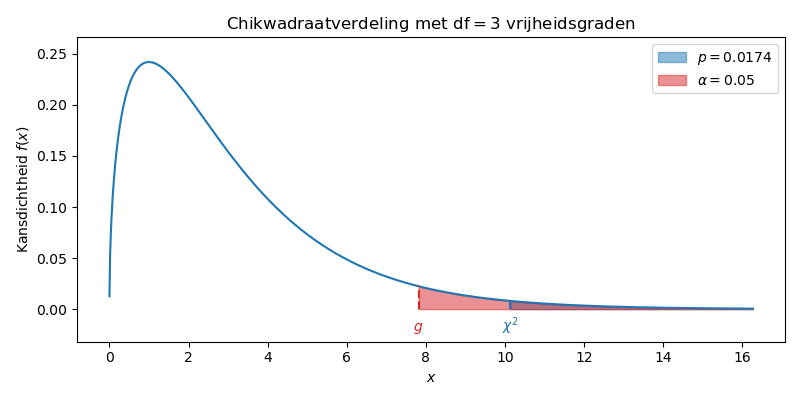
\includegraphics{opg_10.13_p_waarde.png}
        }
    \end{center}

}
